\documentclass[tikz,border=2pt]{standalone}
% ---------------------------------------------------------------------------
% figures/house.tex -- the shared look. Every figure \input's this, so six
% figures look like one hand drew them instead of six.
%
% HOW FIGURES WORK HERE. tikz/pgf is NOT on ACM's production package list, so
% the documents never load it. Each figure is its own standalone document in
% this directory, compiled to a PDF by `make figures`, and pulled into a
% section with
%
%     \begin{figure}
%       \centering
%       \includegraphics{figures/my-figure}
%       \caption{What to LOOK at, not what the figure is of.}
%       \label{fig:my-figure}
%     \end{figure}
%
% Three conventions:
%   * a float sits where it is discussed;
%   * a caption says what to look at, not what the figure is of;
%   * a figure is checked by rendering it and looking, not by a clean compile.
%
% The palette below is the same as the one in preamble.tex. It is repeated
% rather than shared because these are standalone documents that never see the
% paper's preamble, so a colour changed there must be changed here too.
% ---------------------------------------------------------------------------
\usepackage{amsmath}
% The figures build with LuaLaTeX like the documents, so their text is the
% paper's Libertine and their code is the paper's Iosevka.
\usepackage{fontspec}
\setmainfont{LinLibertine_R.otf}[BoldFont=LinLibertine_RB.otf,ItalicFont=LinLibertine_RI.otf,BoldItalicFont=LinLibertine_RBI.otf,Ligatures=TeX]
\setmonofont{Iosevka Custom}[Scale=MatchLowercase,RawFeature={-liga,-calt,-clig,-dlig}]
% Math in the figures is the paper's math: acmart sets Libertinus Math under
% LuaTeX, so the letters on a wire match the letters in the text around it.
\usepackage{unicode-math}
\setmathfont{LibertinusMath-Regular.otf}
\usetikzlibrary{positioning,arrows.meta,fit,backgrounds,calc}

% Blackboard Z, which the documents get from the paper preamble.
% Kept here so a figure never reaches for the paper's preamble.
\newcommand{\Z}{\mathbb{Z}}


\definecolor{ink}{HTML}{16191D}
\definecolor{accent}{HTML}{1F4E79}
\definecolor{accentsoft}{HTML}{E8EEF4}
% accent, accentwarm and accentplum mark the temporary's basis level -- level
% 0, 1, 2 -- wherever a picture or a matrix has to show which branch is which.
\definecolor{accentwarm}{HTML}{9A5B00}
\definecolor{accentplum}{HTML}{8E2F5F}
\definecolor{muted}{HTML}{5B6470}
\definecolor{hairline}{HTML}{C9CFD6}

\tikzset{
  % Every figure inherits this: thin lines, small type, generous air.
  house/.style={
    >={Stealth[length=2.1mm, width=1.6mm]},
    line width=0.5pt,
    node distance=9mm and 15mm,
    every node/.style={font=\small},
  },
  % A thing.
  box/.style={
    draw=ink, line width=0.5pt, rounded corners=1.5pt,
    inner xsep=6pt, inner ysep=4pt, align=center,
  },
  % A thing we are drawing attention to. One per figure, at most.
  boxhi/.style={box, draw=accent, fill=accentsoft, text=ink},
  % A thing that is context, not content.
  boxdim/.style={box, draw=hairline, text=muted},
  % An arrow, and the word on it.
  flow/.style={->, draw=ink},
  flowdim/.style={->, draw=hairline},
  lbl/.style={font=\footnotesize\itshape, text=accent, inner sep=2pt},
  lbldim/.style={font=\footnotesize, text=muted, inner sep=2pt},
  % A dashed grouping rectangle behind a set of nodes.
  group/.style={draw=hairline, dashed, rounded corners=2pt, inner sep=7pt},
}

\begin{document}
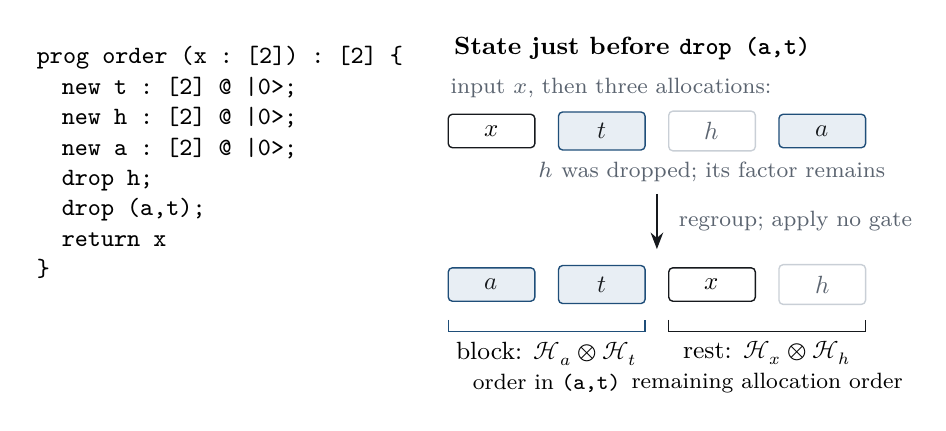
\begin{tikzpicture}[house]
\node[anchor=north west,align=left,font=\small\ttfamily] at (0,0) {prog order (x : [2]) : [2] \{\\
\quad new t : [2] @ |0>;\\
\quad new h : [2] @ |0>;\\
\quad new a : [2] @ |0>;\\
\quad drop h;\\
\quad drop (a,t);\\
\quad return x\\
\}};
\node[anchor=west,font=\small\bfseries] at (5.3,-.15) {State just before \texttt{drop (a,t)}};
\node[anchor=west,lbldim] at (5.3,-.65) {input $x$, then three allocations:};
\node[box,minimum width=11mm] (x) at (5.9,-1.2) {$x$};
\node[boxhi,minimum width=11mm] (t) at (7.3,-1.2) {$t$};
\node[boxdim,minimum width=11mm] (h) at (8.7,-1.2) {$h$};
\node[boxhi,minimum width=11mm] (a) at (10.1,-1.2) {$a$};
\node[lbldim] at (8.7,-1.72) {$h$ was dropped; its factor remains};
\draw[flow] (8,-2.0)--(8,-2.7);
\node[anchor=west,lbldim] at (8.2,-2.35) {regroup; apply no gate};
\node[boxhi,minimum width=11mm] at (5.9,-3.15) {$a$};
\node[boxhi,minimum width=11mm] at (7.3,-3.15) {$t$};
\node[box,minimum width=11mm] at (8.7,-3.15) {$x$};
\node[boxdim,minimum width=11mm] at (10.1,-3.15) {$h$};
\draw[accent] (5.35,-3.6)--(5.35,-3.75)--(7.85,-3.75)--(7.85,-3.6);
\draw[ink] (8.15,-3.6)--(8.15,-3.75)--(10.65,-3.75)--(10.65,-3.6);
\node[align=center] at (6.6,-4.2) {block: $\mathcal H_a\otimes\mathcal H_t$\\\footnotesize order in \texttt{(a,t)}};
\node[align=center] at (9.4,-4.2) {rest: $\mathcal H_x\otimes\mathcal H_h$\\\footnotesize remaining allocation order};
\end{tikzpicture}
\end{document}
